\documentclass{standalone}
\usepackage{tikz}
\usetikzlibrary{patterns, positioning}


\begin{document}
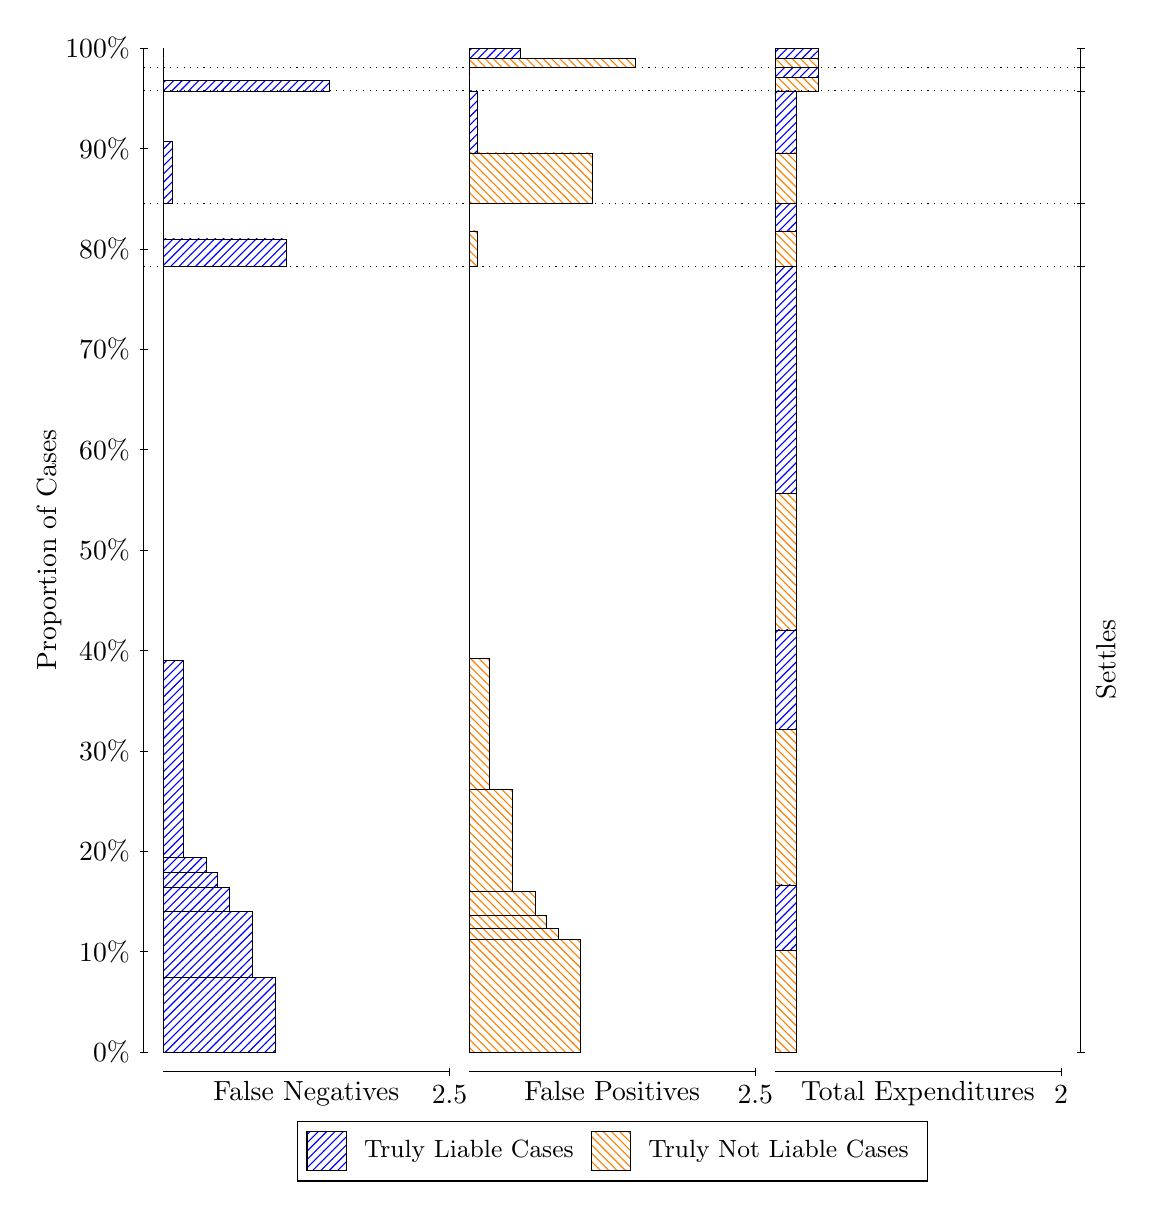
\begin{tikzpicture}
\draw[black, very thin] (1.5,1.75) -- (1.5,14.5);
\node[rotate=90, text=black, anchor=center] at (0.3, 8.125) {Proportion of Cases};
\draw[black, very thin] (1.45,1.75) -- (1.55,1.75);
\node[text=black, anchor=east] at (1.45, 1.75) {0\%};
\draw[black, very thin] (1.45,3.025) -- (1.55,3.025);
\node[text=black, anchor=east] at (1.45, 3.025) {10\%};
\draw[black, very thin] (1.45,4.3) -- (1.55,4.3);
\node[text=black, anchor=east] at (1.45, 4.3) {20\%};
\draw[black, very thin] (1.45,5.575) -- (1.55,5.575);
\node[text=black, anchor=east] at (1.45, 5.575) {30\%};
\draw[black, very thin] (1.45,6.85) -- (1.55,6.85);
\node[text=black, anchor=east] at (1.45, 6.85) {40\%};
\draw[black, very thin] (1.45,8.125) -- (1.55,8.125);
\node[text=black, anchor=east] at (1.45, 8.125) {50\%};
\draw[black, very thin] (1.45,9.4) -- (1.55,9.4);
\node[text=black, anchor=east] at (1.45, 9.4) {60\%};
\draw[black, very thin] (1.45,10.675) -- (1.55,10.675);
\node[text=black, anchor=east] at (1.45, 10.675) {70\%};
\draw[black, very thin] (1.45,11.95) -- (1.55,11.95);
\node[text=black, anchor=east] at (1.45, 11.95) {80\%};
\draw[black, very thin] (1.45,13.225) -- (1.55,13.225);
\node[text=black, anchor=east] at (1.45, 13.225) {90\%};
\draw[black, very thin] (1.45,14.5) -- (1.55,14.5);
\node[text=black, anchor=east] at (1.45, 14.5) {100\%};

\draw[black, very thin] (13.4,1.75) -- (13.4,14.5);
\draw[black, very thin] (13.35,1.75) -- (13.45,1.75);
\node[anchor=west] at (13.35, 1.75) {};
\draw[black, very thin] (13.35,11.725) -- (13.45,11.725);
\node[anchor=west] at (13.35, 11.725) {};
\draw[black, very thin] (13.35,12.53) -- (13.45,12.53);
\node[anchor=west] at (13.35, 12.53) {};
\draw[black, very thin] (13.35,13.956) -- (13.45,13.956);
\node[anchor=west] at (13.35, 13.956) {};
\draw[black, very thin] (13.35,14.256) -- (13.45,14.256);
\node[anchor=west] at (13.35, 14.256) {};
\draw[black, very thin] (13.35,14.5) -- (13.45,14.5);
\node[anchor=west] at (13.35, 14.5) {};

\draw[black, very thin, pattern color=blue, pattern=north east lines] (1.75,1.75) rectangle (3.167,2.7015);
\draw[black, very thin, pattern color=blue, pattern=north east lines] (1.75,2.7015) rectangle (2.8763,3.5314);
\draw[black, very thin, pattern color=blue, pattern=north east lines] (1.75,3.5314) rectangle (2.5857,3.8414);
\draw[black, very thin, pattern color=blue, pattern=north east lines] (1.75,3.8414) rectangle (2.4403,4.0303);
\draw[black, very thin, pattern color=blue, pattern=north east lines] (1.75,4.0303) rectangle (2.295,4.2244);
\draw[black, very thin, pattern color=blue, pattern=north east lines] (1.75,4.2244) rectangle (2.0043,6.7244);
\draw[black, very thin, pattern color=orange, pattern=north west lines] (1.75,6.7244) rectangle (1.75,11.725);
\draw[black, very thin, pattern color=blue, pattern=north east lines] (1.75,11.725) rectangle (3.3123,12.076);
\draw[black, very thin, pattern color=orange, pattern=north west lines] (1.75,12.076) rectangle (1.75,12.53);
\draw[black, very thin, pattern color=blue, pattern=north east lines] (1.75,12.53) rectangle (1.859,13.317);
\draw[black, very thin, pattern color=orange, pattern=north west lines] (1.75,13.317) rectangle (1.75,13.956);
\draw[black, very thin, pattern color=blue, pattern=north east lines] (1.75,13.956) rectangle (3.8573,14.087);
\draw[black, very thin, pattern color=orange, pattern=north west lines] (1.75,14.087) rectangle (1.75,14.256);
\draw[black, very thin, pattern color=orange, pattern=north west lines] (1.75,14.256) rectangle (1.75,14.369);
\draw[black, very thin, pattern color=blue, pattern=north east lines] (1.75,14.369) rectangle (1.75,14.5);
\draw[black, very thin, pattern color=orange, pattern=north west lines] (5.6333,1.75) rectangle (7.0503,3.1754);
\draw[black, very thin, pattern color=orange, pattern=north west lines] (5.6333,3.1754) rectangle (6.7597,3.3181);
\draw[black, very thin, pattern color=orange, pattern=north west lines] (5.6333,3.3181) rectangle (6.6143,3.4806);
\draw[black, very thin, pattern color=orange, pattern=north west lines] (5.6333,3.4806) rectangle (6.469,3.7907);
\draw[black, very thin, pattern color=orange, pattern=north west lines] (5.6333,3.7907) rectangle (6.1783,5.0825);
\draw[black, very thin, pattern color=orange, pattern=north west lines] (5.6333,5.0825) rectangle (5.8877,6.7508);
\draw[black, very thin, pattern color=blue, pattern=north east lines] (5.6333,6.7508) rectangle (5.6333,11.725);
\draw[black, very thin, pattern color=orange, pattern=north west lines] (5.6333,11.725) rectangle (5.7423,12.179);
\draw[black, very thin, pattern color=blue, pattern=north east lines] (5.6333,12.179) rectangle (5.6333,12.53);
\draw[black, very thin, pattern color=orange, pattern=north west lines] (5.6333,12.53) rectangle (7.1957,13.168);
\draw[black, very thin, pattern color=blue, pattern=north east lines] (5.6333,13.168) rectangle (5.7423,13.956);
\draw[black, very thin, pattern color=orange, pattern=north west lines] (5.6333,13.956) rectangle (5.6333,14.124);
\draw[black, very thin, pattern color=blue, pattern=north east lines] (5.6333,14.124) rectangle (5.6333,14.256);
\draw[black, very thin, pattern color=orange, pattern=north west lines] (5.6333,14.256) rectangle (7.7407,14.369);
\draw[black, very thin, pattern color=blue, pattern=north east lines] (5.6333,14.369) rectangle (6.2873,14.5);
\draw[black, very thin, pattern color=orange, pattern=north west lines] (9.5167,1.75) rectangle (9.7892,3.0418);
\draw[black, very thin, pattern color=blue, pattern=north east lines] (9.5167,3.0418) rectangle (9.7892,3.8717);
\draw[black, very thin, pattern color=orange, pattern=north west lines] (9.5167,3.8717) rectangle (9.7892,5.8501);
\draw[black, very thin, pattern color=blue, pattern=north east lines] (9.5167,5.8501) rectangle (9.7892,7.1116);
\draw[black, very thin, pattern color=orange, pattern=north west lines] (9.5167,7.1116) rectangle (9.7892,8.8422);
\draw[black, very thin, pattern color=blue, pattern=north east lines] (9.5167,8.8422) rectangle (9.7892,11.725);
\draw[black, very thin, pattern color=orange, pattern=north west lines] (9.5167,11.725) rectangle (9.7892,12.179);
\draw[black, very thin, pattern color=blue, pattern=north east lines] (9.5167,12.179) rectangle (9.7892,12.53);
\draw[black, very thin, pattern color=orange, pattern=north west lines] (9.5167,12.53) rectangle (9.7892,13.168);
\draw[black, very thin, pattern color=blue, pattern=north east lines] (9.5167,13.168) rectangle (9.7892,13.956);
\draw[black, very thin, pattern color=orange, pattern=north west lines] (9.5167,13.956) rectangle (10.062,14.124);
\draw[black, very thin, pattern color=blue, pattern=north east lines] (9.5167,14.124) rectangle (10.062,14.256);
\draw[black, very thin, pattern color=orange, pattern=north west lines] (9.5167,14.256) rectangle (10.062,14.369);
\draw[black, very thin, pattern color=blue, pattern=north east lines] (9.5167,14.369) rectangle (10.062,14.5);
\draw[black, dotted] (1.5,11.725) -- (13.4,11.725);
\draw[black, dotted] (1.5,12.53) -- (13.4,12.53);
\draw[black, dotted] (1.5,13.956) -- (13.4,13.956);
\draw[black, dotted] (1.5,14.256) -- (13.4,14.256);
\draw[black, very thin] (1.75,1.5) -- (5.3833,1.5);
\node[text=black, anchor=north] at (3.5667, 1.5) {False Negatives};
\draw[black, very thin] (5.3833,1.45) -- (5.3833,1.55);
\node[text=black, anchor=north] at (5.3833, 1.45) {2.5};

\draw[black, very thin] (5.6333,1.5) -- (9.2667,1.5);
\node[text=black, anchor=north] at (7.45, 1.5) {False Positives};
\draw[black, very thin] (9.2667,1.45) -- (9.2667,1.55);
\node[text=black, anchor=north] at (9.2667, 1.45) {2.5};

\draw[black, very thin] (9.5167,1.5) -- (13.15,1.5);
\node[text=black, anchor=north] at (11.333, 1.5) {Total Expenditures};
\draw[black, very thin] (13.15,1.45) -- (13.15,1.55);
\node[text=black, anchor=north] at (13.15, 1.45) {2};

\node[text=black, centered, rotate=90] at (13.72, 6.7376) {Settles};





\draw (7.449999999999999,1.5) node[draw=none] (baseCoordinate) {};
\begin{scope}[align=center]
        \matrix[scale=0.5, draw=black, below=0.5cm of baseCoordinate, nodes={draw}, column sep=0.1cm]{
            \node[rectangle, draw, minimum width=0.5cm, minimum height=0.5cm, pattern color=blue, pattern=north east lines] {}; &
            \node[draw=none, font=\small, text=black] (B) {Truly Liable Cases}; &
            \node[rectangle, draw, minimum width=0.5cm, minimum height=0.5cm, pattern color=orange, pattern=north west lines] {}; &
            \node[draw=none, font=\small, text=black] (B) {Truly Not Liable Cases}; \\
            };
\end{scope}

\end{tikzpicture}
\end{document}